\documentclass{beamer}

\mode<presentation> {
	\usetheme{Antibes}
	\setbeamertemplate{footline}[page number]	
	\setbeamertemplate{navigation symbols}{}
	\setbeamertemplate{items}[square]
}

\usepackage{graphicx}
\usepackage{booktabs}


\title[DragonFly]{Project DragonFly: Vehicle Surveillance System}
\institute[GCEK-CSE]{Department of Computer Science and Engineering \\Government College of Engineering Kannur}
\author[Group 3]{
	{\small \textit{Guided by:}} Dr. Rafeeque P.C \\
	\medskip
	{\small \textbf{\textit{Group 3}}} \\
	Abhinand C \\ Edwin Jose George \\ Lavanya E.V \\ Shilpa Suresh
}
\date{\today}

\begin{document}
	
	%---------------------------------------------------------------------------
	% METADATA -----------------------------------------------------------------
	%---------------------------------------------------------------------------

	\begin{frame}
	\titlepage
	\end{frame}

	\begin{frame}{Table of Contents}
	\tableofcontents
	\end{frame}


	%---------------------------------------------------------------------------
	% INTRODUCTION -------------------------------------------------------------
	%---------------------------------------------------------------------------

	\section{Introduction}
	\subsection{Objective}
	\begin{frame}{Objective}
		
		Policing agencies have setup vast networks of distributed surveillance cameras along major routes. The sheer amount of data generated is overwhelming for manual analysis, to trace routes of rouge vehicles.\\~\\
				
		DragonFly is an AI based project that aims to resolve this particular issue. 
	\end{frame}
	
	\subsection{Proposed System}
	\begin{frame}{Steps}
		\begin{itemize}
			\item The user provides the system with vehicle descriptions such as color, make,
			model, location, time-period etc. 
			\item The system finds corresponding match by making
use of various AI techniques. 
			\item The system tries to re-identify the said vehicle across multiple camera locations.
			\item The system finds the path followed by the said vehicle
along with the detected frame at each camera points.
		\end{itemize}
	\end{frame}
	
	\begin{frame}{Architecture Design}
		\begin{center}
			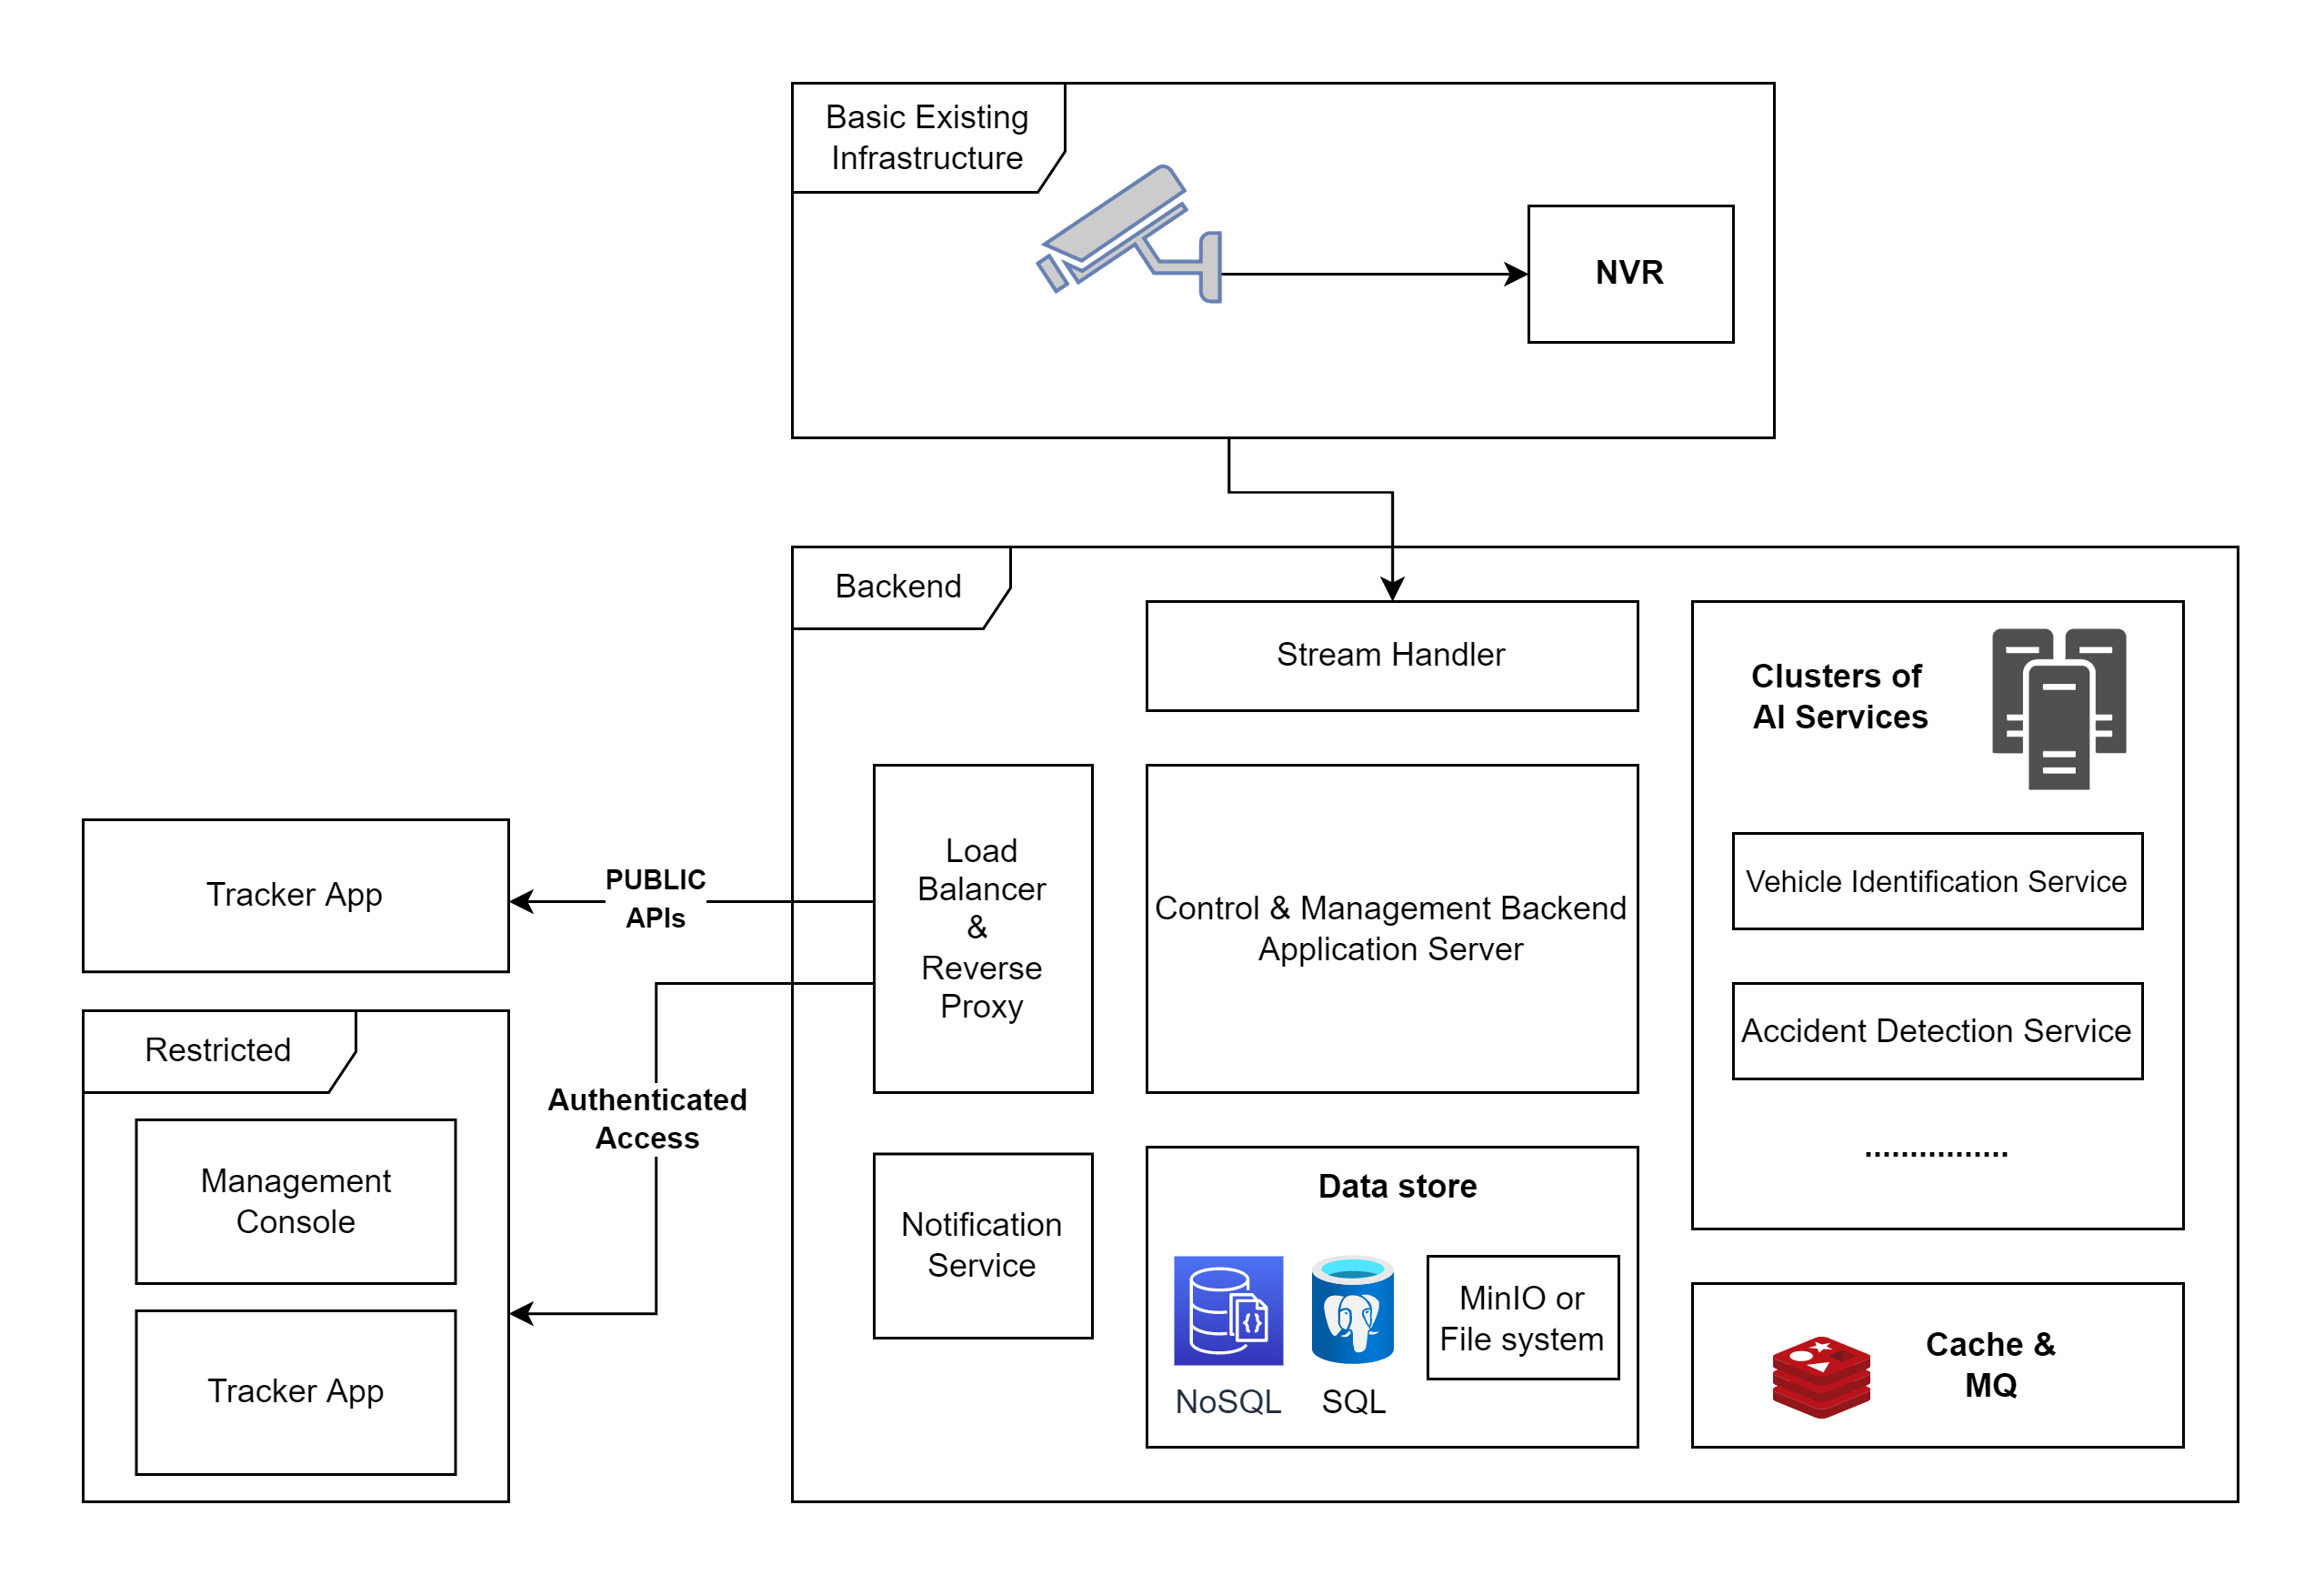
\includegraphics[width=\linewidth]{res/architecture_high_level}
		\end{center}
	\end{frame}

	\begin{frame}{Pipeline1}
		\begin{center}
			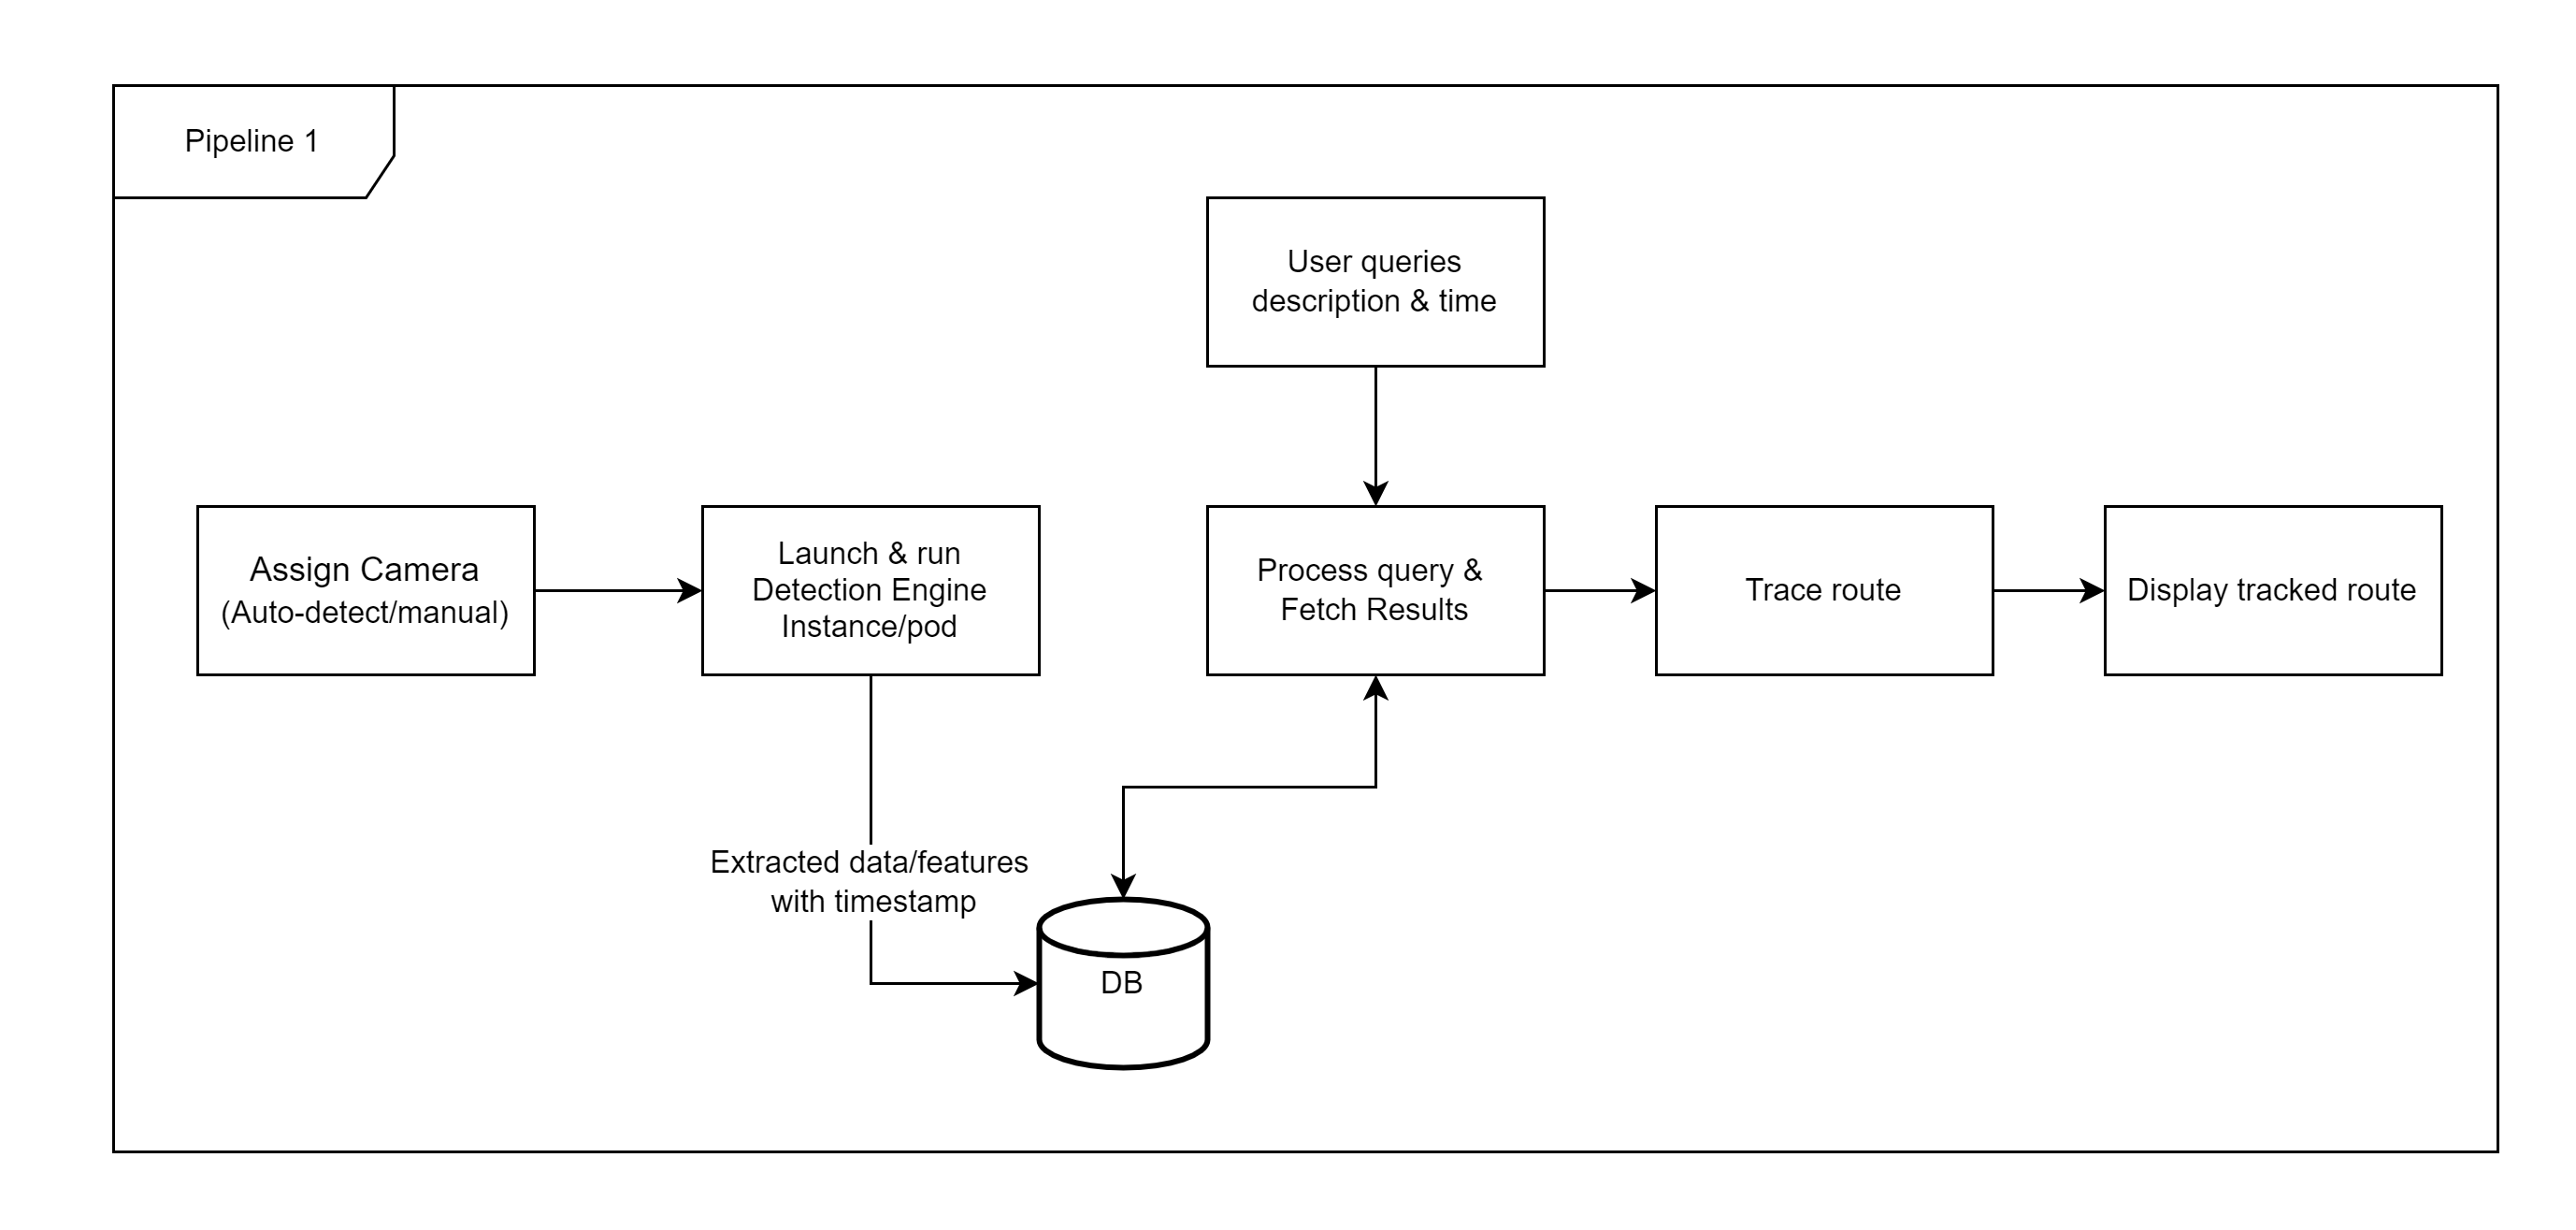
\includegraphics[width=\linewidth]{res/pipeline1}
		\end{center}
	\end{frame}

	\begin{frame}{Pipeline2}
		\begin{center}
			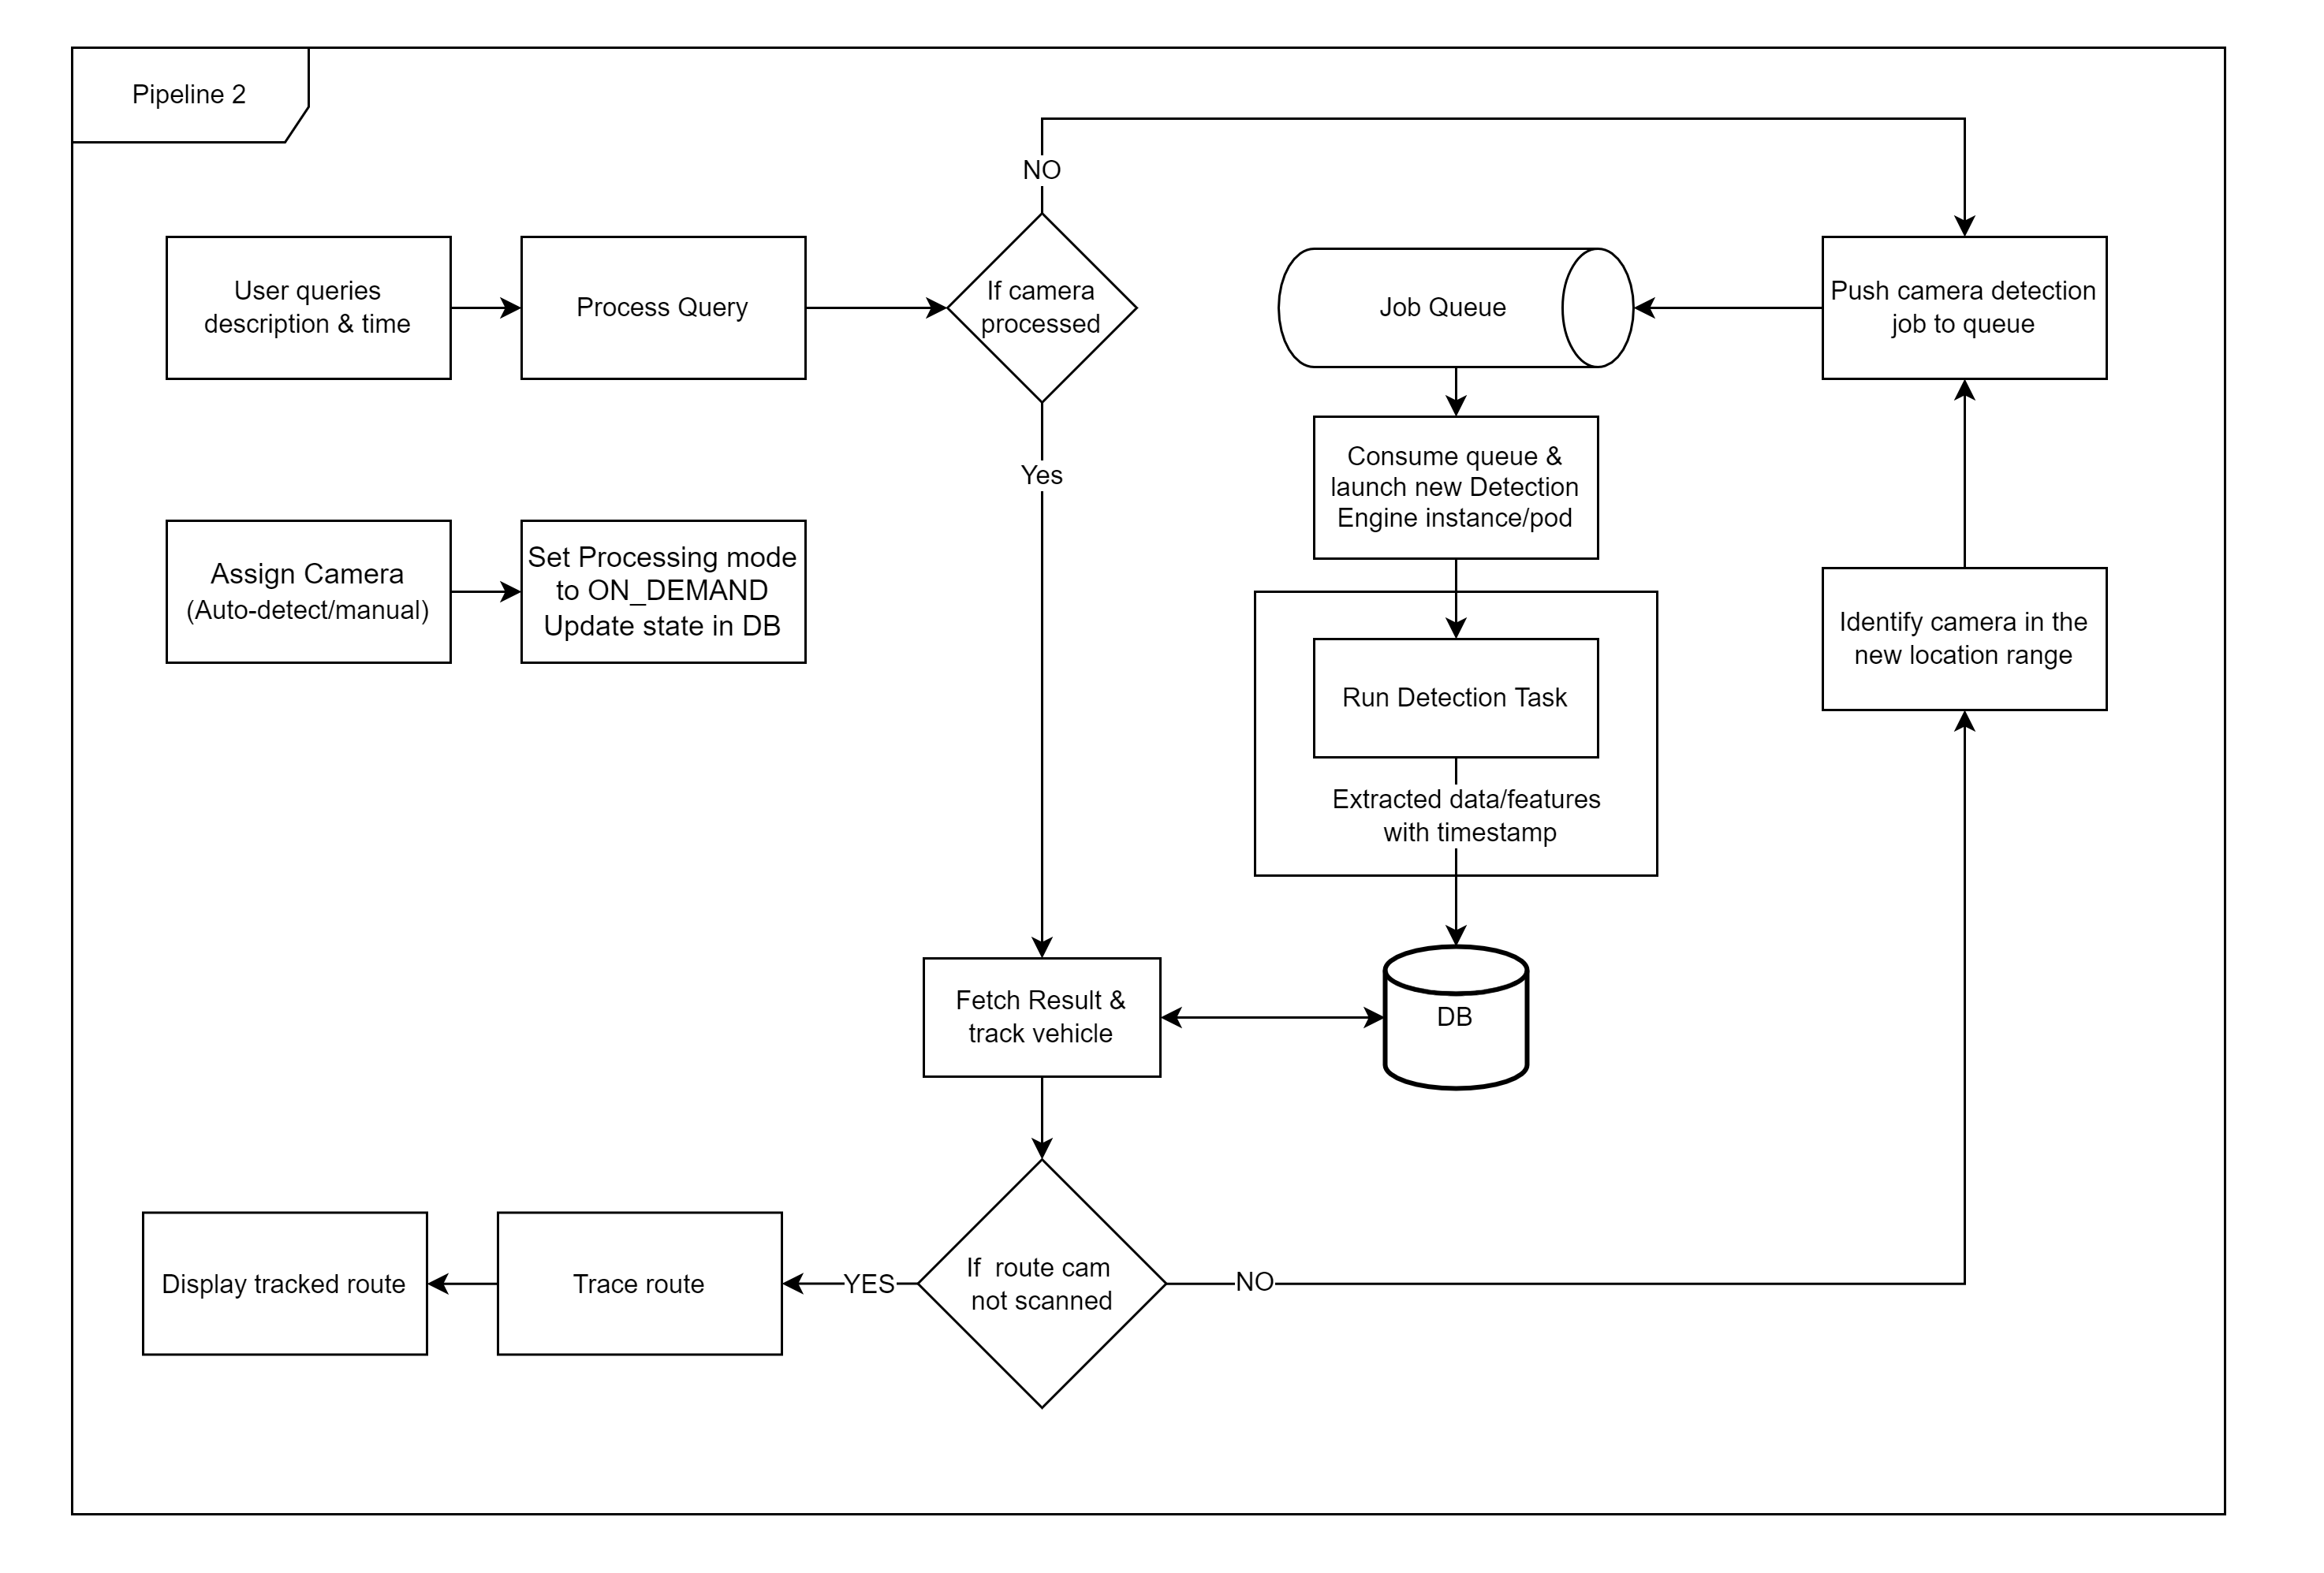
\includegraphics[width=\linewidth]{res/pipeline2}
		\end{center}
	\end{frame}

\end{document} 